% !TEX root = main.tex
\section{Obecny stan i dalszy rozwój narzędzia GenericMonitoringTool}
Narzędzie GenericMonitoringTool jest szeroko i chętnie wykorzystywane w ramach platformy Athena, na potrzeby tworzenia histogramów i monitorowania kodu.
W momencie pisania tej pracy, w jej kodzie zadeklarowanych jest ponad 450 zmiennych monitorowanych w obrębie 53 różnych algorytmów. 
Mogą one wypełnić danymi prawie 4500 zdefiniowanych histogramów.
Do tej pory nie zostały zgłoszone żadne krytyczne błędy, które uniemożliwiałyby pracę z tym narzędziem.

Obecnie toczą się prace nad dodawaniem nowych funkcjonalności do kodu GenericMonitoringTool.
Mają one na celu pokrycie dodatkowych przypadków użycia, dzięki którym możliwe będzie dotarcie do większej liczby użytkowników. 
Został on również szeroko wykorzystany podczas technicznego "reprocessingu" dla 22 wersji platformy Athena, dla którego przykładowe histogramy zostały przedstawione na \figref{fig:athena:histogram_TH1}, \figref{fig:athena:histogram_TH1_time} i \figref{fig:athena:histogram_TH2}.

\begin{figure}[!ht]
\centering
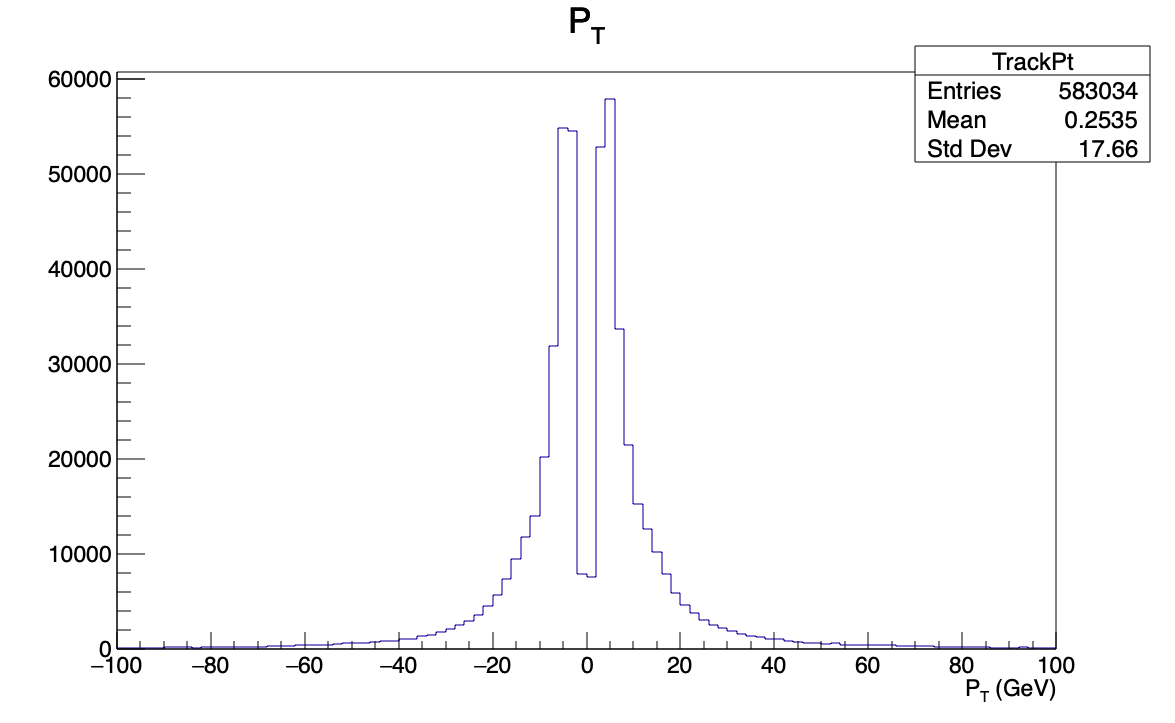
\includegraphics[width=1\textwidth]{img/histogram_TH1.png}
\caption{
Przykładowy histogram TH1 dla zmiennej monitorowanej typu 'Scalar', utworzony z pomocą GenericMonitoringTool.
}
\label{fig:athena:histogram_TH1}
\end{figure}

\begin{python}[caption=TH1 Scalar, label={lst:athena:histogram_TH1}]
#TODO
\end{python}

\begin{figure}[!ht]
\centering
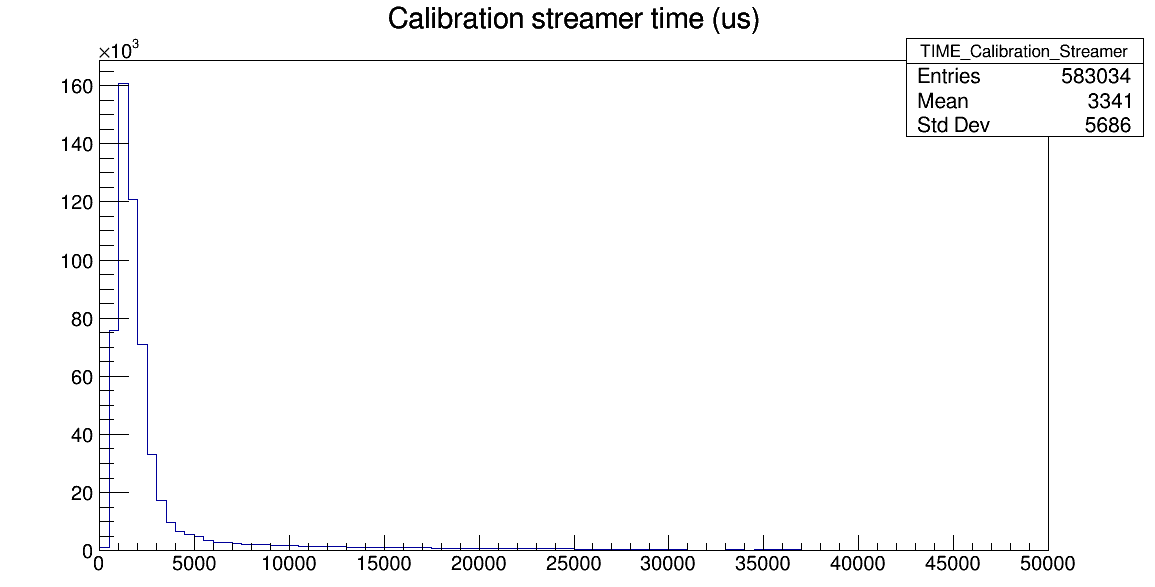
\includegraphics[width=1\textwidth]{img/histogram_TH1_time.png}
\caption{
Przykładowy histogram TH1 dla zmiennej monitowanej typu 'Timer', utworzony z pomocą GenericMonitoringTool 
}
\label{fig:athena:histogram_TH1_time}
\end{figure}

\begin{python}[caption=TH1 Time, label={lst:athena:histogram_TH1_time}]
#TODO
\end{python}

\begin{figure}[!ht]
\centering
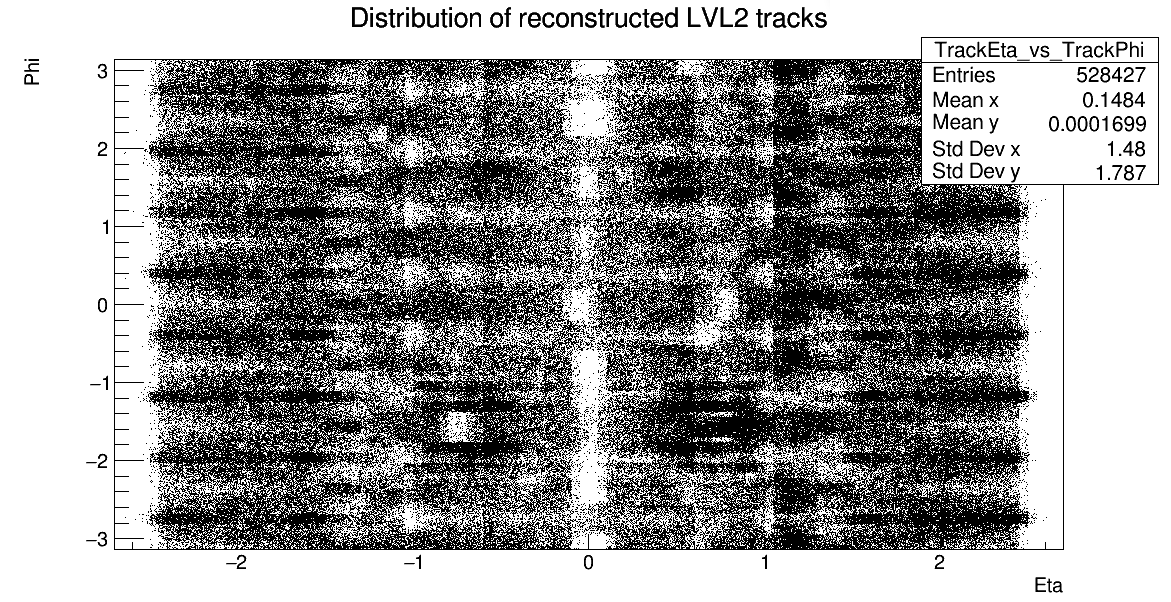
\includegraphics[width=1\textwidth]{img/histogram_TH2.png}
\caption{
Przykładowy histogram TH2 dla dwóch zmiennych monitowanych typu 'Scalar', utworzony z pomocą GenericMonitoringTool 
}
\label{fig:athena:histogram_TH2}
\end{figure}

\begin{python}[caption=TH2 Scalar, label={lst:athena:histogram_TH2}]
#TODO
\end{python}

W przyszłości, planowana jest m.in. aktualizacja framworka ROOT.
Jego najnowsze wersje zapewniają bezpieczeństwo dla przetwarzania wielowątkowego i wieloprocesowego. 
Taka zmiana pozwoli usunąć niepotrzebne sekcje krytyczne z kodu GenericMonitoringTool.

\subsection{Zastosowanie w systemie online}
//TODO
\subsection{Zastosowanie do monitorowania offline - Data Quality}
//TODO~\cite{atlas-multithread-article}